\chapter{Results\label{ch:results}}

\epigraph{I pass with relief from the tossing sea of Cause and Theory to the firm ground of Result
and Fact.} {\textit{Winston S. Churchill, The Story of the Malakand Field Force}}

In this chapter we look at the expermental results of the system, both piecewise and as a whole.
We start by summarizing the hardware that the benchmarks is ran on in \cref{sec:results-hw}. In
\cref{ch:res-ops} we look at the overhead of the operations done by CMR\@. In \cref{sec:results-ds} we
look at the performance of the data structuers implemented, with and without the overehead CMR, and
compare them to alternatives in the Rust ecosystem, like Crossbeam~\cite{crossbeam} and data
structures in the standard library wrapped in a \code{Mutex}.

\clearpage

\section{Hardware\label{sec:results-hw}}

We start this chapter by looking at the hardware the benchmark suite is ran on.  The benchmark
suite is ran on four separate machines: one desktop machine \gribb{}, an ARM based cloud server
\scaleway{} and two quad-socket high-end server CPUs, \mitserver{} and \daslab{}.  The four CPUs
all have different indented usage and price range, with the exception of the two high-end servers.
It is therefore interesting to look at the performance on all systems, as oposed to limiting
ourselfes to a certain price range or intended usage.

\gribb{} is an x86 desktop CPU running at 3.40GHz, with 4 cores and 8 threads. The system has 16 GB of
RAM, and is the system with the least abount of free memory.

\scaleway{} is an ARMv8 CPU at 2.50GHz, having 32 cores and 32 threads over two NUMA cores, with 32
GB of RAM\@.

\mitserver{} is an x86 CPU for the server market running 10 cores with 20 threads at 2.40GHz. The
system we ran tests on was a quad socket system, making the total thread count 80. The system had 1
TB of main memory.

\daslab{}, the last server, is similar to the \mitserver{} except that it has a slightly fast clock
rate, 2.70GHz, and it has 18 cores with a total of 36 cores. This was also a quad-core system,
making the total thread count a whopping 144. The system used had 512 GB of main memory.


The number of threads for the benchmark ranges from 1 to slightly above the number of hardware
threads on the CPU the benchmark is ran on. It is expected that the performance evens out when the
number of threads reaches the maximum number of hardware threads in all benchmarks. The duration of
the benchmarks also varies, due to memory constraints of the system they are ran on.


\section{Operations of CMR\label{ch:res-ops}}

The operations that CMR provides that are most interesting to look at is allocation
(\code{cmr::alloc}) and guard initialization and destruction (\code{guard!}), as these operations
are the only ones that have any significant overhead. Atomic loads pointer manipulations are mainly
tricks of the type system to ensure the safey of the operations, and has no run-time overhead.


\subsection{Primitives}

We begin by looking at the performance of \code{Guard} construction and allocation.  The generated
code from the \code{guard!} macro contains some initialization checks, which the compiler could not
remove despite constructing multiple guards in a row. For this reason the \code{guards!} macro were
written, which reduced the execution time by 20\% for 10 declarations.  We measure the time one
\code{Guard} declaration takes, and the time for 10 \code{Guard}s to be declared using the
\code{guards!} macro.  All measurements are amortized over 1000 runs as shown in
\cref{lst:guard-bench}, but the reported numbers are per operation.

\begin{figure}[ht]
\begin{lstlisting}[style=Rust]
#[bench]
fn cmr_guard_1k(b: &mut Bencher) {
    global_init();
    let _t = ::test::test_init();
    b.iter(|| for _ in 0..1000 { guard!(g);
                                 let _: &mut Guard<u64> = g; }); }
\end{lstlisting}
  \caption{Benchmark for \code{Guard} construction.\label{lst:guard-bench}}
\end{figure}

The results for all machines are summarized in \cref{tb:ops-perf}.
Note that a single \code{guard!} is faster than \code{guards!} per declaration. This can be
attributed to that destruction of a \code{Guard} must find itself in the \code{Vec} of
\code{Guard}s, so more \code{Guard}s take longer.

\begin{table}[ht]
  \centering
  \caption{Summary of the execution of selected CMR operations. All numbers are per single
  operation.\label{tb:ops-perf}}
\begin{tabular}{l r r r r}
  Machine & \code{guard!} & \code{guards!} & \code{cmr::alloc} & \code{Box::new} \\
  \toprule
  \scaleway{}  & 78 ns & 92 ns & 335 ns & 185 ns \\
  \midrule
  \gribb{}     & 13 ns & 13 ns &  45 ns &  28 ns \\
  \midrule
  \mitserver{} & 28 ns & 30 ns & 73 ns & 50 ns \\
  \midrule
  \daslab{}    & 12 ns & 18 ns & 56 ns & 33 ns\\
  \bottomrule
\end{tabular}
\end{table}



\section{Data Structures\label{sec:results-ds}}


As mentioned in \cref{ch:usage}, the stack and the queue both have operational bottlenecks;
that is most operations contest the same memory locations, which causes poor scaling with more
cores. In addition, since the list from \cref{sec:usage-list} is the primary building block for the
hash table, we do not look at the performance of the list explicitly. Thus, the only remaining
data structure to look at is the hash table. This is also the most interesting.

We compare the four hashmap variations:
\begin{enumerate*}[1)]
  \item the hashmap from \cref{sec:usage-hashmap} (\code{cmr})
  \item the same hashmap, but with all operations of CMR to be no-ops (\code{cmr(noop)})
  \item an external SkipList implementation from the Crossbeam project~\cite{crossbeam-skiplist}
    (\code{cb}) and
  \item \code{std::HashMap} wrapped in a \code{Mutex} (\code{std}).
\end{enumerate*}

The \code{HashMap} benchmarks consists of four operations: \code{insert}, \code{remove},
\code{contains}, and a combination of the three: a 80/10/10 split of \code{contains},
\code{inserts}, and \code{remove} respectively. This is shown experimentally to mirror real world
\todo{cite !!}
usage of hashmaps quite well, and is common in concurrent performance testing.

Naturally, this is not quite an apples-to-apples comparison; the hashmap of CMR is implemented
quite differently than in Crossbeam, and even more different than the one in the standard library.
Therefore we can, and should, attribute parts of any experimental difference to the difference in
implementation.


\clearpage
\subsection{\gribb}

\begin{figure}[ht]
  \centering
  \hmgrid{gribb}
  \caption{HashMap performance on \gribb}
\end{figure}

The experimental results reveal that the hash table scales properly up to the thread limit of the
machine. As mentioned in \cref{sec:results-hw} this is expected. We also see that the variant of
CMR with all overhead removed performs strictly better than the real CMR\@; this acts as a fine
sanity check. Crossbeams SkipList also scales well, although its performance is slightly lower than
that of CMR, with the expection of the very last data points from the \code{remove} benchmark.

It is also nice to see that the na\"\i{}ve approach of wrapping a \code{HashMap} in a \code{Mutex}
scales rather poorly; however we should point out that for Crossbeam, it makes sense to use the
\code{Mutex} with up to four threads; which, for many applications, might be sufficient.

\clearpage
\subsection{\scaleway}

The \scaleway is of a different nature than the remaining CPUs in this section, since it is an ARM
machine. It also has a relative low clock speed. This manifests itself here in that the throughput
in terms of absolute numbers is lower than the \gribb{} on multiple benchmarks, despite having four
times the thread count.

In the \code{insert} benchmark we see a dip in throughput at 16 cores. This may be attributed to
the number of threads being too high to run effectively on a single socket. However, if we
calculate how many elements are inserted, we get $5M \times 16 = 80M$ elements; since the size of
the pointer array is only $\approx 1M$,  we get a load factor of $\approx 80$, which means that
inserts risk looking at 80 nodes before finding the correct place in the list to insert!
In addition, the \code{remove} benchmark seems not to run into this problem. This suggests that it
is in fact the capacity of the hash table that is the limiting factor, and not the cross-socket
synchronization.

\begin{figure}[ht]
  \centering
  \hmgrid{scw}
  \caption{HashMap performance on \scaleway}
\end{figure}


\clearpage
\subsection{\mitserver{} and \daslab{}}

\begin{figure}[ht]
  \begin{minipage}[h]{\linewidth}
    \centering
    \hmgrid{eecs-ath-16}
    \caption{HashMap performance on \mitserver{}}
  \end{minipage}
  \begin{minipage}[h]{\linewidth}
    \centering
    \hmgrid{dasquad}
    \caption{HashMap performance on \daslab{}}
  \end{minipage}
\end{figure}

This section contains both the \mitserver{} and the \daslab{}; this is done due to the similarities
of both the CPUs and of the data.

The \code{HashMap} performance on the quad sockets is much more pessimistic than the graphs from
the earlier sections; the operational throughput on both \code{insert} and \code{remove} evens out
already after 16 and 36 cores for the \mitserver{} and \daslab{} respectively. This is probably
because of the fact that only a limited numebr of threads are running on one socket, so that any
shared memory loction that is modified by the \code{HashMap}s operations must be flushed to main
memory. For us, this is the number of elements in the \code{HashMap}, which we need for resizing
approproately.

A back of the envelope calculation supports this claim: The \mitserver{} runs at $\SI{2400}{GHz}$,
and with 16 threads we manage about $4M$ \code{insert}s per second in total. This means that if we
assume that all accesses to the \code{count} field happend sequentially, each access takes
$\frac{\SI{2400}{GHz}}{4M} = 600$ cycles per operation. While this is a lot for a single memory
access, it is not too far off from main memory access latencies, which are often around
$\SI{100}{ns}$~\cite{memlatency}.

Yet another observation which supports the claim is that \code{contains} seems unaffected by the
NUMA effects, as it does not mutate the \code{HashMap} in any way.



\clearpage
\section{Allocator}

The choice of allocator is also shown to have a real effect. \cref{fig:jemalloc-diff} shows the
\code{HashMap::insert} benchmark while using the JeMalloc allocator (drawn lines) and the default
system allocator (dashed lines).
JeMalloc is optimized for multiple threads; however in this benchmark we clearly see a large
increase in favour of the system allocator with 32 threads. This lead is however unique for all
other data points, with the exception of a few of the data points from the Crossbeam hash table,
when the thread count is 96, 128, and 144.

The general trend for the system allocator for both variants of CMR is downwards from its maxima at
16 threads, while neither allocator seems to affect the hash table from Crossbeam.
This might mean that the allocation is not in the bottleneck for Crossbeam, whereas it is for the
hash table implemented using CMR\@.

\begin{figure}[ht]
  \centering
  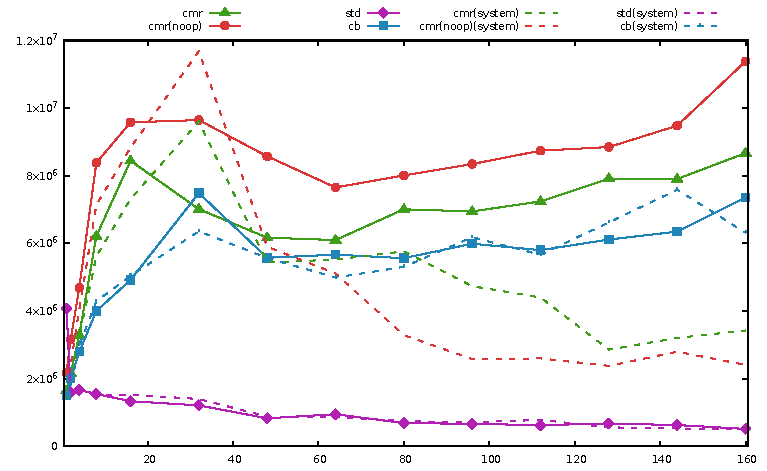
\includegraphics{graphs/jemalloc-difference}
  \caption{The \code{HashMap} insert benchmark using JeMalloc and the system allocator\label{fig:jemalloc-diff}}
\end{figure}
